%%%%%%%%%%%%%%%%%%%%%%%%%%%%%%%%%%%%%%%%%%%%%%%%%%%%%
%%% Task 1 %%%%%%%%%%%%%%%%%%%%%%%%%%%%%%%%%%%%%%%%%%
%%%%%%%%%%%%%%%%%%%%%%%%%%%%%%%%%%%%%%%%%%%%%%%%%%%%%
\task{Deflecting magnet}

%%%%%%%%%%%%%%%%%%%%%%%%%%%%%%%%%%%%%%%%%%%%%%
\taskGerman{Ablenkmagnet}
%%%%%%%%%%%%%%%%%%%%%%%%%%%%%%%%%%%%%%%%%%%%%%

A dipole magnet with an axial cross-section as shown in \autoref{fig:dipol_magnet} is used to deflect the particle beam of charged heavy ions in a particle accelerator. A rated direct current $I_{\mathrm{n}} = \SI{5000}{\ampere}$ flows through the two excitation coils. The copper conductors of the coil winding are directly water-cooled due to the high current density of $J = \SI{18}{\ampere\per\milli\metre^2}$.

\begin{germanblock}
    Ein Dipolmagnet mit einem axialen Querschnitt nach \autoref{fig:dipol_magnet} wird zur Ablenkung des Teilchenstrahls geladener schwerer Ionen in einem Teilchenbeschleuniger verwendet. Durch die beiden Erregerspulen fließt ein Bemessungsgleichstrom $I_{\mathrm{n}} = \SI{5000}{\ampere}$. Die Kupferhohlleiter der Spulenwicklung sind wegen der hohen Stromdichte von $J = \SI{18}{\ampere\per\milli\metre^2}$ direkt wassergekühlt.
\end{germanblock}

\begin{figure}[h!]
    \centering
    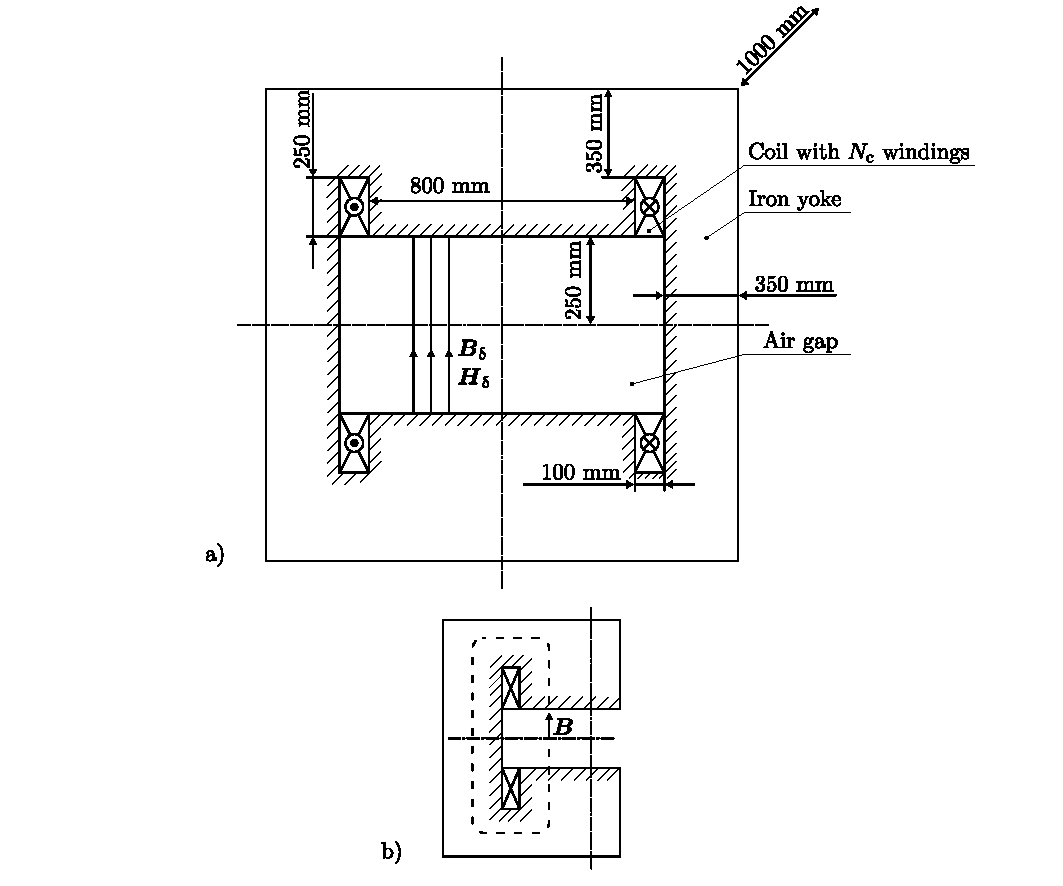
\includegraphics{fig/sketch_dipol_magnet.pdf}
    \caption{Sketch of the deflecting magnet a) and an idealized field line b).}
    \label{fig:dipol_magnet}
\end{figure}



\subtask{How large is the magnetic field in the air gap, when there is a homogeneous magnetic flux density of $B_{\updelta} = \SI{3.141}{\tesla}$? How many windings per coil $N_{\mathrm{c}}$ are necessary? Neglect the magnetization effort of the iron yoke.}{3}
\begin{hintblock}
    If you have not found a solution for the number of winding turns in this subtask, continue with $N_{\mathrm{c}} = 140$. 
\end{hintblock}
\subtaskGerman{Wie groß ist die magnetische Feld im Luftspalt, wenn dort eine homogene Flussdichte von $B_{\updelta} = \SI{3,141}{\tesla}$ herrscht? Wie groß ist die erforderliche Windungszahl $N_{\mathrm{c}}$ der Spulen? Vernachlässigen Sie den Magentisierungsbedarf des Eisenjochs.}
\begin{germanhintblock}
    Wenn Sie in dieser Teilaufgabe keine Lösung für die Anzahl der Windungen gefunden haben, fahren Sie mit $N_{\mathrm{c}} = 140$ fort.
\end{germanhintblock}


\begin{solutionblock}
    The relationship between the magnetic flux density $B_{\updelta}$ and the magnetic field is given by:
    $$ H_{\updelta} = \frac{B_{\updelta}}{\mu_0} = \frac{\SI{3.141}{\tesla}}{\SI{4\pi 10^-7}{\volt\second\per\ampere\per\metre}} = \SI{2499528}{\ampere\per\metre}.$$

    The general form of Ampère's circuital law is defined as 
    $$ \oint_{\partial S} \bm{H} \cdot \mathrm{d}\bm{s} = \sum_k \theta_k$$

    which can be simplified based on the made assumptions:
    $$\theta_{\updelta} = l_{\updelta} H_{\updelta} = \SI{500}{\milli\metre} \cdot \SI{2499528}{\ampere\per\metre} = \SI{1249764}{\ampere}. $$

    The given magneto static situation is represented with
    $$ \sum_{k}^{} \theta_{k} = N I,$$
    which leads to the number of winding turns:
    $$ N_{\mathrm{c}} = \frac{\theta_{\updelta}}{I} = \frac{\SI{1249764}{\ampere}}{\SI{2\cdot5}{\kilo\ampere}} = 124.97,$$
    therefore, 125 turns are selected.

\end{solutionblock}


\subtask{How lare is the magnetic flux in the air gap?}{1}
\subtaskGerman{Wie groß ist der Luftspaltfluss?}

\begin{solutionblock}
    The magnetic flux is calculated by
    $$ \phi_{\updelta} = B_{\updelta} A_{\updelta} = \SI{3.141}{\tesla} \cdot \SI{(0.8\cdot 1)}{\metre^2} = \SI{2.51}{\weber},$$
    where the surface is taken from the sketch in \autoref{fig:dipol_magnet}.

\end{solutionblock}

\subtask{Calculate the magnetic flux density $B_{\mathrm{Fe}}$ in the iron yoke. Therefore, neglect magnetic leakage fluxes.} {1}
\subtaskGerman{Berechnen Sie die magentische Flussdichte $B_{\mathrm{Fe}}$ in dem Eisenjoch. Vernachlässigen Sie dafür alle magnetischen Streuflüsse.}


\begin{solutionblock}
    Since the leakage fluxes are neglected, the flux $\phi_{\updelta}$ in the air gap and the $\phi_{\mathrm{Fe}}$ in the iron yoke are equal. Thus
    $$ \phi_{\updelta} = \phi_{\mathrm{Fe}} = B_{\mathrm{Fe}} A_{\mathrm{Fe}} = B_{\updelta} A_{\updelta},$$
    which results into:
    $$B_{\mathrm{Fe}} = \frac{A_{\updelta}}{A_{\mathrm{Fe}}} B_{\updelta} = \frac{\SI{(0.8\cdot1)}{\metre^2}}{\SI{2\cdot(0.35\cdot1)}{\metre^2}} \cdot \SI{3.141}{\tesla} = \SI{3.59}{\tesla}.$$

\end{solutionblock}



\subtask{The average length of the iron yoke is given with $l_{\mathrm{Fe}} = \SI{1.2}{\metre}$. How large is the magnetization effort of the iron yoke, when the permeability $\mu_{\mathrm{Fe}} = 126 \mu_0$? Is the assumption of zero magnetization effort from subtask 1 correct?}{2}

\subtaskGerman{Die mittlere Länge des Eisenjochs beträgt $l_{\mathrm{Fe}}=\SI{1,2}{\metre}$. Wie groß ist der Magentisierungsbedarf des Eisens, wenn die Permeabiliät $\mu_{\mathrm{Fe}} = 126 \mu_0$ beträgt? Ist die Vernachlässigung des Eisenmagnetisierungsbedarfs für die Bestimmung des Erregerbedarfs aus Teilaufgabe 1 zulässig?}

\begin{solutionblock}
    With the calculated flux density in the previous task and the given information of $\mu_{\mathrm{r}}$, the magnetic field is calculated as
    $$ H_{\mathrm{Fe}} = \frac{B_{\mathrm{Fe}}}{\mu_0 \mu_{\mathrm{r}}} = \frac{B_{\mathrm{Fe}}}{126 \mu_0} = \frac{\SI{3.59}{\tesla}}{\SI{126 \cdot 4 \pi 10^{-7}}{\volt\second\per\ampere\per\metre}} = \SI{22673}{\ampere\per\metre},$$

    which results into the magnetic voltage of:
    $$ \theta_{\mathrm{Fe}} = H_{\mathrm{Fe}} \cdot l_{\mathrm{Fe}} = \SI{22673}{\ampere\per\metre} \cdot \SI{1.2}{\metre} = \SI{27208}{\ampere}. $$

    The comparison between the magnetic voltage between the iron yoke and the air gap results in
    $$ \frac{\theta_{\mathrm{Fe}}}{\theta_{\updelta}} = \frac{\SI{27208}{\ampere}}{\SI{1249764}{\ampere}} = 0.022, $$
    which is very small and, therefore, the assumption from subtask 1 is valid.
    
\end{solutionblock}


\subtask{How lage is the electrical resistance of the excitation coil at $\SI{50}{\celsius}$ with an average winding length $l_{\mathrm{w}}=\SI{4}{\metre}$  and an electrical conductivity of $\kappa_{\mathrm{Cu}}=\SI{50\cdot10^6}{\siemens\per\metre}$?}{2}
\subtaskGerman{Wie groß ist bei $\SI{50}{\celsius}$ und einer mittleren Windingslänge $l_{\mathrm{w}}=\SI{4}{\metre}$ der elektrische Widerstand der Erregerwicklung bei einer elektrischen Leitfähigkeit $\kappa_{\mathrm{Cu}}=\SI{50\cdot10^6}{\siemens\per\metre}$?}

\begin{solutionblock}
    The cross section of the conductor is given by
    $$ q_{\mathrm{Cu}} = \frac{I_{\mathrm{n}}}{J} = \frac{\SI{5000}{\ampere}}{\SI{18}{\ampere\per\milli\metre^2}} = \SI{277.8}{\milli\metre^2},$$

    whichs results in the resistance per coil as follows:
    $$ R_{\mathrm{c}} = \frac{1}{\kappa_{\mathrm{Cu}}} \frac{N_{\mathrm{c}}l_{\mathrm{w}}}{q_{\mathrm{Cu}}} = \frac{1}{\SI{50\cdot 10^6}{\siemens\per\metre}}\frac{125 \cdot \SI{4}{\metre}}{\SI{277.8}{\milli\metre^2}} = \SI{0.036}{\Omega}. $$
\end{solutionblock}


\subtask{Calculate the necessary voltage $U$ and the excitation losses $P_{\mathrm{l}}$.}{2}
\subtaskGerman{Berechnen Sie die nötige Spannung $U$ und die Erregerverluste $P_{\mathrm{l}}$.}

\begin{solutionblock}
    The necessary voltage is calculated with:
    $$ U = R I_{\mathrm{n}} = 2 R_{\mathrm{c}} I_{\mathrm{n}} = \SI{0.072}{\Omega}\cdot \SI{5000}{\ampere} = \SI{360}{\volt}. $$

    The resulting loss is determined by:
    $$ P_{\mathrm{l}} = R I_{\mathrm{n}}^2 = 2 R_{\mathrm{c}} I_{\mathrm{n}}^2 = \SI{0.072}{\Omega} \cdot (\SI{5000}{\ampere})^2 = \SI{1.8}{\mega\watt}. $$
\end{solutionblock}


\subtask{Calculate the flux linkage $\psi_{\mathrm{coil}}$ of one coil.}{1}
\subtaskGerman{Berechnen Sie den verketteten Fluss von einer Spule $\psi_{\mathrm{coil}}$.}

\begin{solutionblock}
    The flux linkage of one coil is calculated by:
    $$ \psi_{\mathrm{coil}} = N \phi_{\mathrm{coil}} = N \phi_{\updelta} = 125 \cdot \SI{2.51}{\volt\second} = \SI{313.8}{\volt\second}.$$
\end{solutionblock}

\subtask{How large is the inductivity $L$, when the two coils are connected in series?}{1}
\subtaskGerman{Wie groß ist die Wicklungsinduktivität $L$, wenn die Spulen in Serie geschaltet sind?}

\begin{solutionblock}
    The inductivity for one coil is given with
    $$L_{\mathrm{c}} = \frac{\psi_{\mathrm{coil}}}{I_{\mathrm{n}}} = \frac{\SI{313.8}{\volt\second}}{\SI{5000}{\ampere}} = \SI{62.8}{\milli\henry},$$

    and, results in the total inductivity of:
    $$ L = 2 L_{\mathrm{c}} = 2 \cdot \SI{62.8}{\milli\henry} = \SI{125.6}{\milli\henry}.$$
\end{solutionblock}